\section{Relevant concepts and assumptions}\label{sec:relevant-concepts}

In this section, we review relevant concepts like predictable DTNs, onion routing and key management that we consider essential to understand our proposal.

\subsection{Predictable DTNs overview}

Predictable DTNs are such networks where the behaviour is known in advance or where a repetitive action occurs over time.

% dtn-book: 
These networks fit perfectly with the concept of oracle schemes. Oracle schemes are a subset of DTN routing protocols. In this schemes there is a set of nodes that have nearly full knowledge of the network and its planned evolution \cite{dtn-book}. There are oracles that can answer any question regarding contacts between two nodes at any point in time, this oracles are called contacts oracle \cite{oracle-types}. Contacts oracle schemes are used in deterministic scenarios where the oracle node have full details of occurred contacts as well as the future ones.

For instance, we could consider public transport networks as predictable (deterministic) networks because every node performs the same route periodically so this route can be known in advance. This information could be shared among all nodes in the network in order to let them be "oracle", i.e: let them have full knowledge of the whole network. It is important to note that, despite these networks are nearly deterministic, an error needs to be assumed for exceptional situations.

As we explained previously, contact information will be known by everyone, therefore a security analysis needs to be carried out. This analysis is discussed in section \ref{sec:sanalysis}.

\subsection{Onion routing overview}

We provide a high-level description of how onion routing works. The source node, wishing to send an anonymous message to another node, chooses a path ciphering the message several times making "layers". Onion routing uses a pre-shared symmetric key between the source and a node on the path to make this layers. When the message reaches a node, the layer is removed with the pre-shared key. At the end of the process, if every node in the path did the decryption correctly, the destination will receive the fully decrypted message without knowing who sent it.

\begin{figure}[hbt]
  \centering
  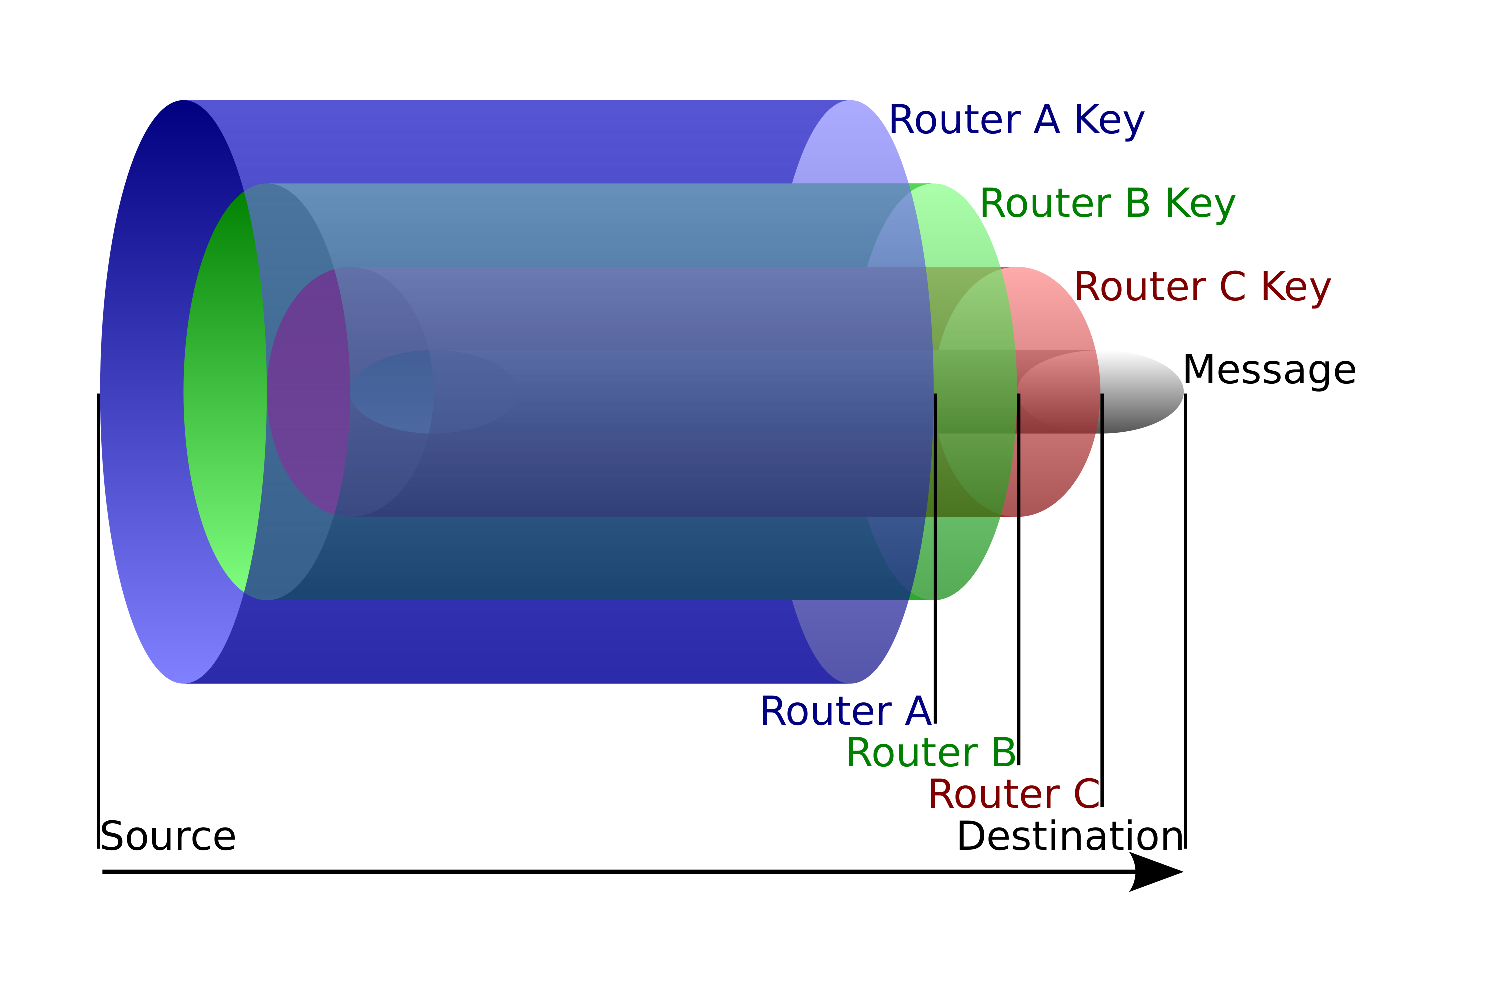
\includegraphics[scale=0.35]{imgs/onion}
  \caption{Onion routing graphical example of how layering works \cite{wiki-onion-routing-image}.}
  \label{fig:dtn-example}
\end{figure}

To clear out the main idea, an example can be seen in figure \ref{fig:dtn-example}. The source node wants to send an anonymous message to a destination using a previously chosen path composed by the nodes A, B and C. The source ciphers the message with the corresponding pre-shared symmetric key of C, B and A respectively. When the message reaches every hop, each node removes the external layer using the key. Finally, the destination will get the fully decrypted message.

\subsection{Key management}

In order to use onion routing a prior key exchange process needs to be performed. We consider that the loading of the network information behaviour as well as the keys sharing process will be done simultaneously at a previous stage, i.e: before starting the periodical routing. For example, in public transport networks the data as well as the needed keys will be shared before the scheduled route starts.
